\usepackage{listings}
\usepackage{xcolor}
\chapter{GPU Programming Patterns} \label{chap:GPU_programming_patterns}
接下來,我們將討論在廣泛的 GPU 應用中常用的 GPU 程式設計模式。對於每種討論的程式設計模式,我們將涵蓋相關數據結構的佈局,並回顧對數據執行的常見指令。我們將提供HIP編寫的程式範例,使讀者能夠熟練地識別和利用這些程式設計模式在他們的GPU程式中。

\section{二維 kernels}
GPU 是由數千個核心組成的大規模平行架構。因此, GPU 非常適合數據平行計算。由於二維 kernel 模式通常是數據平行的,這使我們能夠利用 GPU 發揮其固有的平行性。處理大量數據矩陣的任務,如圖像處理和機器學習應用,可以透過將任務分佈到這些核心上計算而顯著加速。

當我們在二維 grid 中處理數據時,通常有相鄰的元素彼此依賴。許多科學和工程模擬包含在二維空間中處理數據。當今的 GPU 架構非常適合解決二維問題並處理二維數據。在開發利用二維 kernel 的應用程式時,開發人員能夠針對特定計算任務和 GPU 硬體配置優化他們的程式碼。這種層級的優化可以帶來顯著的速度提升。

在本節中,我們將探討一個使用二維 block 進行矩陣乘法的 HIP 程式碼\cite{Gilbert2009Linear}。在深入了解矩陣乘法的 HIP 程式碼之前,我們將回顧矩陣乘法通常是如何計算的。假設我們有兩個矩陣,A 和 B。矩陣 A 有 m 列和 n 行,矩陣 B 有 n 列和 k 行。在這種情況下,結果矩陣 C 將有 m 列和\hl{k 行}。


% %New colors defined below
% \definecolor{codegreen}{rgb}{0,0.6,0}
% \definecolor{codegray}{rgb}{0.5,0.5,0.5}
% \definecolor{codepurple}{rgb}{0.58,0,0.82}
% \definecolor{backcolour}{rgb}{0.95,0.95,0.92}
% %Code listing style named "mystyle"
% \lstdefinestyle{mystyle}{
%   backgroundcolor=\color{backcolour}, commentstyle=\color{codegreen},
%   keywordstyle=\color{magenta},
%   numberstyle=\tiny\color{codegray},
%   stringstyle=\color{codepurple},
%   basicstyle=\ttfamily\footnotesize,
%   breakatwhitespace=false,         
%   breaklines=true,                 
%   captionpos=t,                    
%   keepspaces=true,                 
%   numbers=left,                    
%   numbersep=5pt,                  
%   showspaces=false,                
%   showstringspaces=false,
%   showtabs=false,                  
%   tabsize=2
% }
%  Listing 5.1: 矩陣乘法的cpu實作
%"mystyle" code listing set
% \lstset{style=mystyle}
\begin{lstlisting}[language=c++,caption={矩陣乘法的cpu實作}]
#include <iostream>
#define N 32
void cpu_matrix_multiplication(
float *a, float *b, float *result, int n) {
    for (int i = 0; i < n; ++i) {
        for (int j = 0; j < n; ++j) {
            int tmp = 0;
            for (int k = 0; k < n; ++k) {
                tmp += a[i * n + k] * b[k * n + j];
            }
            result[i * n + j] = tmp;
        }
    }
}

 int main(){
     float *a, *b, *c;
     a = (float*)malloc(sizeof(float)*N*N);
     b = (float*)malloc(sizeof(float)*N*N);
     c = (float*)malloc(sizeof(float)*N*N);
    
    //初始化矩陣 A
    for (int i = 0; i < N; ++i) {
        for (int j = 0; j < N; ++j) {
            a[i * N + j] = rand() % RAND_MAX;
        }
    }
    //初始化矩陣 B
    for (int i = 0; i < N; ++i) {
        for (int j = 0; j < N; ++j) {
            b[i * N + j] = rand() % RAND_MAX;
        }
    }
    cpu_matrix_multiplication(a, b, c, N);
    return 0;
}
\end{lstlisting}


為了計算矩陣 A 和矩陣 B 的乘積,我們首先將矩陣 A 的第一列與矩陣 B 的第一行進行內積。這將得到結果矩陣中的第一個元素。我們對矩陣 A 和矩陣 B 的所有列與行重複此過程,以獲得完整的結果矩陣。這是一個兩個 N x N 矩陣的矩陣乘法,其中 N 定義為 32;因此,將進行 32³ = 32,768 次乘法運算和 32² × (32 − 1) = 31,744 次加法運算。接下來,我們將看看一個使用 CPU 進行矩陣乘法的實作,以便更好地理解這個過程。



這段程式碼(見 Listing 5.1)使用 CPU 計算兩個方形矩陣相乘。它包含一個名為 \texttt{cpu\_matrix\_multiplication} 的函數,該函數接受三個浮點數變數的指標,其中 \texttt{a} 和 \texttt{b} 代表要相乘的矩陣,\texttt{result} 指向儲存乘法結果的矩陣。整數 \texttt{n} 指定矩陣的大小。 \texttt{cpu\_matrix\_multiplication} 函數使用巢狀 for 迴圈來乘兩個輸入矩陣。外層兩個迴圈遍歷結果矩陣的列和行,最內層的迴圈計算結果的每個元素。乘法是透過遍歷矩陣 \texttt{a} 的列索引和矩陣 \texttt{b} 的行索引,將對應元素相乘並將結果加到一個臨時變數中來完成的。每個輸出結果的計算是獨立的。一旦最內層的迴圈完成,臨時變數將被儲存到結果矩陣的對應元素中。主函數使用 \texttt{rand()} 函數以隨機值初始化兩個矩陣 \texttt{a} 和 \texttt{b}。然後,呼叫 \texttt{cpu\_matrix\_multiplication} 函數來執行矩陣乘法並將結果存儲在矩陣 \texttt{c} 中。



為了在這個例子的基礎上進一步,我們將研究使用 HIP 開發的兩個方形矩陣相乘實作。首先需要注意的是,必須包含使用 HIP 運行時調用所需的標頭檔。我們還添加了矩陣大小和每個 grid 中 block 數量的巨集,分別設置為 16 和 256。(見 Listing 5.2)。

%"mystyle" code listing set
\lstset{style=mystyle}
%  Listing 5.2: 標頭檔和巨集
\begin{lstlisting}[language=c++,caption={標頭檔和巨集}]
#include <hip∕hip_runtime.h>
#define BLOCK_SIZE 16
#define N 256
\end{lstlisting}


仔細查看 HIP \textbf{kernel}(見 Listing 5.3),我們可以看到該\textbf{kernel}的目的是對方陣進行矩陣乘法。這個\textbf{kernel}預期四個輸入參數:指向矩陣 a、b 和 c 的指標,以及方陣的大小 N。


該kernel的結構設計使得每個處理 thread 負責計算結果矩陣中的一個單獨元素。特定 block 內的每個 thread 由 threadIdx.x 和 threadIdx.y 索引,而 grid 內的每個 block 則分別由 blockIdx.x 和 blockIdx.y 在 x 軸和 y 軸上。


接下來,我們將變數 sum 初始化為零。這個變數將用來累加選定列和行中的元素。然後,我們使用 if 語句檢查列和行索引是否超過矩陣的實際列數和行數。這樣做是為了防止thread執行超出矩陣範圍的操作。


這個 kernel 內的 for 迴圈使用矩陣 a 的一列和矩陣 b 的一行來計算內積。經過求和後,結果會被儲存在矩陣 c 的相應索引中。

%"mystyle" code listing set
%  Listing 5.3: GPU程式碼
\lstset{style=mystyle}
\begin{lstlisting}[language=c++,caption={GPU程式碼}]
__global__ void gpu_matrix_multiplication(float *a,float *b, float *c,
int n){
    int row = blockIdx.y * blockDim.y + threadIdx.y;
    int col = blockIdx.x * blockDim.x + threadIdx.x;
    int sum = 0;
    if( col < n && row < n) {
        for(int i = 0; i < n; i++) {
        sum += a[row * n + i] * b[i * n + col];
        }
        c[row * n + col] = sum;
    }
}
\end{lstlisting}


仔細查看 CPU 程式碼(見 Listing 5.4),我們宣告了具有整數數據類型的指標變數。我們還分配 host 記憶體給矩陣 \texttt{h\_a}、\texttt{h\_b} 和 \texttt{h\_c} 。在這一步之後,我們在 host 上初始化矩陣 \texttt{h\_a} 和 \texttt{h\_b},並用隨機數字填充這些矩陣。

%"mystyle" code listing set
\lstset{style=mystyle}
%  Listing 5.4: CPU 記憶體分配矩陣初始化
\begin{lstlisting}[language=c++,caption={CPU 記憶體分配矩陣初始化}]
int main(){
    float *h_a,*h_b,*h_c,*h_cc;
    h_a =(float*)malloc(sizeof(float)*N*N);
    h_b =(float*)malloc(sizeof(float)*N*N);
    h_c =(float*)malloc(sizeof(float)*N*N);

    //初始化矩陣 A
    for (inti =0; i< N;++i){
        for (int j=0; j <N;++j){
            h_a[i* N+j]= rand()% RAND_MAX;
        }
    }
    //初始化矩陣 B
    for (int i =0; i<N;++i){
        for (intj=0; j<N;++j){
            h_b[i *N+ j]= rand()% RAND_MAX;
        }
    }
\end{lstlisting}


在下一步中,我們在 GPU 上分配記憶體,並將 CPU 的數據複製到 GPU 上作為輸入矩陣(見 Listing 5.5)。接下來,我們啟動kernel函數(見 Listing 5.6),但首先我們需要確定每個 block 的 thread 數量和每個 grid 的 block 數量。為此,我們使用一種稱為 dim3 的數據類型。在我們的例子中,我們創建了一個 \texttt{BLOCK\_size} 乘以 \texttt{BLOCK\_size} 的 grid ,初始時將 \texttt{BLOCK\_size} 設置為 16。因此,block的數量 \texttt{n\_blocks} 透過將 N 除以 \texttt{BLOCK\_size} 計算得到,其中 N 是矩陣的大小。我們使用 ceil 函數將結果向上取整到下一個整數。這使我們能夠創建比實際需要更多的thread,並透過在 kernel 函數中使用 if 語句來避免對矩陣進行不必要的操作。最後,我們使用 hipDeviceSynchronize 確保 GPU 在 CPU 繼續之前完成其工作,防止數據訪問衝突。

%"mystyle" code listing set
\lstset{style=mystyle}
%  Listing 5.5: GPU 記憶體分配與資料傳輸(host到device)
\begin{lstlisting}[language=c++,caption={GPU 記憶體分配與資料傳輸(host到device)}]
int *d_a, *d_b, *d_c;
hipMalloc((void **) &d_a, sizeof(float)*N*N);
hipMalloc((void **) &d_b, sizeof(float)*N*N);
hipMalloc((void **) &d_c, sizeof(float)*N*N);

hipMemcpy(d_a, h_a, sizeof(float)*N*N, hipMemcpyHostToDevice);
hipMemcpy(d_b, h_b, sizeof(float)*N*N, hipMemcpyHostToDevice);
\end{lstlisting}

%"mystyle" code listing set
\lstset{style=mystyle}
%  Listing 5.6: kernel啟動
\begin{lstlisting}[language=c++,caption={kernel啟動}]
dim3threadsPerBlock (BLOCK_SIZE, BLOCK_SIZE);
int n_blocks =ceil(N∕BLOCK_SIZE);
dim3blocksPerGrid (n_blocks, n_blocks);

gpu_matrix_multiplication<<<blocksPerGrid,threadsPerBlock>>>(d_a, d_b,d_c, N);
hipDeviceSynchronize();
\end{lstlisting}


在 kernel 函數執行完畢後,我們可以使用 hipMemcpy 將結果從 GPU 上的 device 結果矩陣 \texttt{d\_c} 複製回 CPU,就像之前一樣(見 Listing 5.7)。將數據移回 CPU 後,我們驗證結果。然後,釋放在 CPU 和 GPU 中分配的記憶體,並返回 0 表示程式已成功運行。

%"mystyle" code listing set
\lstset{style=mystyle}
%  Listing 5.7: 資料傳輸(host到device)和記憶體釋放
\begin{lstlisting}[language=c++,caption={資料傳輸(host到device)和記憶體釋放}]
    hipMemcpy(h_c, d_c, sizeof(float)*N*N, hipMemcpyDeviceToHost);
    hipFree(d_a);
    hipFree(d_b);
    hipFree(d_c);
    free(h_a);
    free(h_b);
    free(h_c);
    return 0;
}
\end{lstlisting}
\section{Stencils}
% 模版運算

Stencil operations代表了另一類重要的極易平行化的演算法。 Stencils 是一類根據鄰近項目迭代更新陣列中數據的演算法。Stencil演算法常用於物理模擬和偏微分方程中,以支持圖像處理的卷積運算。透過應用不同的圖像卷積 kernel(不要與 GPU kernel混淆),該演算法可以平滑和銳化圖像特徵並檢測邊緣。因此,圖像卷積被用於卷積神經網絡(CNN)。


正如在伽瑪校正範例中所討論的,圖像卷積也是極易平行化的 workload 。當映射到 GPU 上時,每個 thread 計算單個像素輸出;因此,不需要在 thread 之間溝通更新。


然而,圖像卷積和伽瑪校正之間存在一些根本性的差異。對於伽瑪校正,所有亮度值被視為獨立值,我們不需要關心它們在圖像中的位置。因此,我們只是將整個圖像作為一個陣列來處理,因此,相對像素位置變得重要。我們使用與卷積kernel形狀相匹配的二維grid,這大大簡化了實作。一般而言, stencil workload 可以是一維、二維或三維的。

%"mystyle" code listing set
\lstset{style=mystyle}
%  Listing 5.8: HIP 平滑運算程式
\begin{lstlisting}[language=c++,caption={HIP 平滑運算程式}]
#include <hip/hip_runtime.h>

#include <vector>

#include "image.h"

__global__ void conv2d(uint8_t *image, float *mask, int image_width,
                       int image_height, int mask_width, int mask_height) {
    int x = blockIdx.x * blockDim.x + threadIdx.x;
    int y = blockIdx.y * blockDim.y + threadIdx.y;

    if (x >= image_width || y >= image_height) {
        return;
    }

    float sum = 0;
    for (int i = 0; i < mask_width; i++) {
        for (int j = 0; j < mask_height; j++) {
            // 計算要讀取的像素座標。
            int image_x = x + i - mask_width / 2;
            int image_y = y + j - mask_height / 2;

            // 避免讀取超出影像範圍的數據。
            if (image_x < 0 || image_x >= image_width || image_y < 0 ||
                image_y >= image_height) {
                continue;
            }

            // 累加像素值。
            int image_index = image_y * image_width + image_x;
            int mask_index = j * mask_width + i;
            sum += image[image_index] / 255.0f * mask[mask_index];
        }
    }

    int image_index = y * image_width + x;
    image[image_index] = sum * 255;
}

int main() {
    int width, height, channels;
    static const int maskWidth = 200;
    static const int maskHeight = 200;
    std::vector<float> mask(maskWidth * maskHeight * channels);
    for (int i = 0; i < maskWidth * maskHeight; ++i) {
        mask[i] = 1.0f / maskWidth / maskHeight / channels;
    }

    // 從磁碟載入影像。

    // 分配 GPU 記憶體並將數據複製到 GPU
    uint8_t *d_image;
    float *d_mask;
    hipMalloc(&d_image, width * height * channels * sizeof(uint8_t));
    hipMalloc(&d_mask, maskWidth * maskHeight * channels * sizeof(float));
    hipMemcpy(d_image, image, width * height * channels * sizeof(uint8_t),
              hipMemcpyHostToDevice);
    hipMemcpy(d_mask, mask.data(),
              maskWidth * maskHeight * channels * sizeof(float),
              hipMemcpyHostToDevice);

    // 計算 grid 大小並啟動 kernel 。
    dim3 block_size = {16, 16, 1};
    dim3 grid_size = {(width + block_size.x - 1) / block_size.x,
                      (height + block_size.y - 1) / block_size.y, 1};
    conv2d<<<grid_size, block_size>>>(d_image, d_mask, width, height, maskWidth,
                                      maskHeight);
    hipDeviceSynchronize();

    // 將數據複製回 host 。
    hipMemcpy(image, d_image, width * height * channels * sizeof(uint8_t),
              hipMemcpyDeviceToHost);

    // 將影像儲存到磁碟。
    hipFree(d_image);
    hipFree(d_mask);
    return 0;
}
\end{lstlisting}


在我們的下一個程式碼範例中,我們展示了一段執行圖像平滑的程式碼。這個kernel中最值得注意的技術是使用二維grid。在host程式中,我們不是使用單個整數來表示 grid 的大小,而是使用包含三個值的 dim3 來表示每個維度上基於 block 的 work items數。由於我們希望使用二維 grid ,我們將 z 維度大小設置為一,並根據我們的問題大小指定 x 和 y 維度。


在kernel函數中,我們必須獲取 x 和 y 兩個維度的 thread ID 。為了獲取這些值,我們使用 threadIdx.x 和 threadIdx.y 操作。 block 維度和 ID 在每個維度中均有定義的相關變數,如範例中所示。

\section{Multi-Kernel 範例- BFS} 
% 多核範例 - BFS

在本章的下一個範例中,我們首先研究廣度優先搜尋(BFS)演算法的 HIP 實作。這個 workload 是 Rodinia
 benchmark suite 的一部分 \cite{Shuai2009Rodinia。BFS 是一種圖搜尋演算法,廣泛應用於路徑尋找、點對點網絡和全球定位系統(GPS)導航等多種應用中。


 BFS 是一種逐層演算法,會在進入下一層之前先探索給定圖層或層級的所有節點。例如,為了避免重複處理同一節點,BFS 使用佇列來標記節點為“已訪問”,如圖 5.1(a) 所示。


\begin{figure}
    \centering
    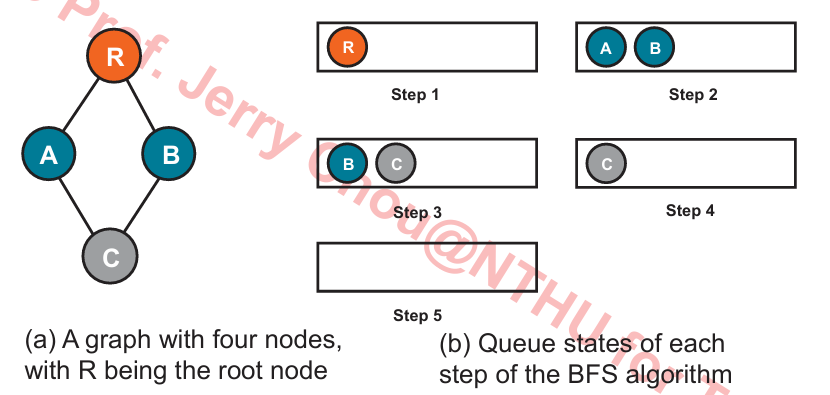
\includegraphics[width=1\linewidth]{FileAusiliari//Screenshots/Figure5-1.png}
    \caption{BFS 演算法的圖示,其中包含四個節點。}
    \label{fig:enter-label}
\end{figure}
% (a)四個節點的圖,其中 R 是根節點   (b)BFS 演算法每一步的佇列狀態



圖 5.1(b) 展示了佇列的處理方式。從根節點 R 開始,我們首先在步驟 1 中標記 R 並將其放入佇列。由於這是根節點,此層級沒有其他節點存在。因此,將 R “彈出”佇列並處理連接的節點 A 和 B。我們將 A 和 B 推入佇列並在步驟 2 中標記為已訪問。之後,由於此層級沒有更多節點需要處理。佇列的頭部 A 彈出,並處理其鄰居。點 A 連接到節點 C 和 R。節點 R 已經被訪問過。因此,節點 C 被推入佇列並在步驟 3 中標記為已訪問。按照這個過程,我們耗盡了節點 A 的所有鄰居。因此,佇列中的下一個項目 B 在步驟 4 中被離隊,佇列中僅剩下節點 C。節點 B 連接到節點 C 和 R,而節點 R 和 C 已經被標記為已訪問。因此,我們不會重新訪問它們。最終,我們到達一個階段,節點 C 是佇列中最後一個元素,並且它連接到的節點 A 和 B 均已經被訪問過。因此,節點 C (最後一個元素)被從佇列中移除。此時,佇列終於為空,如步驟 5 所示。因此,演算法終止。


現在我們已經介紹了 BFS 的基本概念,我們將研究其在 GPU 上的平行實作。這裡展示的實作來自 Rodinia benchmark suite。


該實作旨在找出從給定起始節點到圖中所有頂點所需的最小邊數。所有在給定層級處理的節點通稱為“邊界”(frontier)。應用程式的兩個 kernel 透過使用 DO-WHILE 迴圈連續執行,每個實例代表處理給定層級的節點。節點和邊分別儲存在變數 \texttt{g\_graph\_nodes} 和 \texttt{g\_graph\_edges} 中。變數 \texttt{g\_graph\_mask} 對所有節點(除了根節點)初始化為 FALSE,用於確定下一次 DO-WHILE 迴圈中要處理哪些節點。使用變數 \texttt{g\_cost} 追蹤從前一個節點訪問下一個節點的成本。每當訪問到給定節點的鄰居時,\texttt{g\_cost} 會跟著更新。此外,變數 \texttt{g\_updating\_graph\_mask} 在開始時被初始化為 FALSE。這個變數用來決定第二個kernel必須更新哪些節點的資訊。


在 kernel 1 中,第 5 行,我們檢查 thread ID 是否在圖的範圍內並且是否屬於當前邊界。如果兩個條件都滿足, thread 透過將變數 \texttt{g\_graph\_mask} 設置為 FALSE 將自己從邊界中移除。接下來,我們遍歷該節點的所有鄰居,檢查未訪問的鄰近節點(第 11 行和第 12 行)。對於所有未訪問的鄰居,thread 更新 cost 陣列中的對應 entry。處理過的鄰居透過將 \texttt{g\_updating\_graph\_mask} 設置為 TRUE 來標記,以便第二個 kernel 能夠接著更新它。


在kernel 2 中,我們首先檢查 thread ID 是否在圖的範圍內,並根據 \texttt{g\_updating\_graph\_mask}更新節點。如果條件為 TRUE,該節點會被添加到邊界 Listing 並標記為已訪問。請注意,若節點在\texttt{g\_graph\_mask} 中設置為 TRUE,下一次 DO-WHILE 迴圈將在 kernel 1 中處理這個節點,因為它屬於下一層級。變數 \texttt{g\_over} 設為 TRUE,通知 CPU 再次運行 DO-WHILE 迴圈。


敏銳的讀者可能會想知道為什麼實作了兩個 kernel。與多種 GPU 程式語言類似,HIP 不保證 thread 執行的順序。想象一下,如果一個 thread 在第一個 kernel 的第 11 行 IF 語句中將 \texttt{g\_graph\_mask} 設置為 TRUE 會發生什麼情況。同一 kernel 中的另一個 thread 可能會觸發條件 5 為 TRUE,並在當前層級的所有節點完成之前開始處理下一層級的節點。這將導致潛在的錯誤。回想一下, BFS 的目的是逐層或按層級地搜尋圖。同樣地,如果我們在第一個 kernel 的同一個 IF 語句中將一個節點標記為已訪問,另一個與該節點共享邊的 thread ,即使必須更新 cost 陣列,仍會在第一個 kernel 的第 11 行觸發 FALSE 條件。因此,這個實作需要兩個 kernel 來避免發生“race condition”。


當達到終止條件時,由於沒有更多未訪問的節點,代表所有圖的層級都已被遍歷。因此,我們可以保證 kernel 2 中的所有 thread 都不會觸發第 5 行的 IF 條件。因此,\texttt{g\_over} 將保持為 FALSE,最終終止 DO-WHILE 迴圈和搜尋。

%"mystyle" code listing set
\lstset{style=mystyle}
%  Listing 5.9: BFS的kernel1
\begin{lstlisting}[language=c++,caption={BFS的kernel1}]
__global__ void
Kernel(Node* g_graph_nodes, int* g_graph_edges, bool* g_graph_mask, bool* g_updating_graph_mask, bool *g_graph_visited, int* g_cost, int no_of_nodes)
{
    int tid = hipBlockIdx_x * MAX_THREADS_PER_BLOCK + hipThreadIdx_x;
    if (tid < no_of_nodes && g_graph_mask[tid]) {
        g_graph_mask[tid] = false;
        for (int i = g_graph_nodes[tid].starting; i < (g_graph_nodes[tid].no_of_edges + g_graph_nodes[tid].starting); i++) {
            int id = g_graph_edges[i];
            if (!g_graph_visited[id]) {
                g_cost[id] = g_cost[tid] + 1;
                g_updating_graph_mask[id] = true;
            }
        }
    }
}
\end{lstlisting}

%"mystyle" code listing set
\lstset{style=mystyle}
%  Listing 5.10: BFS的kernel2
\begin{lstlisting}[language=c++,caption={BFS的kernel2}]
__global__ void
Kernel2(bool* g_graph_mask, bool* g_updating_graph_mask, bool* g_graph_visited, bool* g_over, int no_of_nodes)
{
    int tid = hipBlockIdx_x * MAX_THREADS_PER_BLOCK + hipThreadIdx_x;
    if (tid < no_of_nodes && g_updating_graph_mask[tid]) {
        g_graph_mask[tid] = true;
        g_graph_visited[tid] = true;
        *g_over = true;
        g_updating_graph_mask[tid] = false;
    }
}
\end{lstlisting}
\section{CPU-GPU 計算 – KMeans}
% CPU-GPU 計算 – KMeans


雖然在處理數據平行的 workload 時,GPU 可以提供高效能,但對於那些無法輕易平行化且較不理想的 workload ,GPU 可能並不適合。然而,一些演算法結合了平行和串行部分。在這種情況下,一個合理的解決方案是讓 CPU 負責串行部分,而 GPU 負責平行部分。我們需要來回搬動數據,以實作 CPU-GPU 協同計算。


KMeans 是一個具有平行部分和串行部分的 workload 。它是一種廣泛使用的無監督機器學習演算法,旨在對數據進行群集。它根據數據的特徵將一組數據點分成 k 個組(群集)來工作。每個群集由其中心點(稱為質心)特徵化。該演算法將每個數據點分配到最近的質心,從而創建彼此相似數據點的群集。這個過程包含反復更新質心並重新分配數據點到群集,直到群集穩定且不會有顯著改變。儘管 KMeans 假設群集是圓形的,並且在處理複雜群集形狀或不同大小的群集時可能會遇到困難,由於其簡單性和高效性, KMeans 仍被頻繁使用。


KMeans 的訓練過程從初始化階段開始,選擇 k 個初始質心。這種選擇可以是隨機的,也可以基於特定的試探方法,以優化起始位置。一旦這些初始質心確定,演算法就會將數據集中每個數據點分配到最近的質心。這種分配通常依賴於計算每個數據點與每個質心之間的歐氏距離,將每個數據點分配到最近的質心。因此, k 個群集開始圍繞這些質心形成。


在分配階段之後, KMeans 更新每個群集的質心。每個質心的新位置是透過計算分配給該群集的所有數據點的平均值(均值)來確定的。這一步實際上將質心移動到群集內所有數據點的中心位置,優化其在下一次迭代中的位置。


接著,演算法透過檢查質心是否已經穩定下來判斷是否達到收斂。可以透過檢查分配給群集的數據點在連續迭代中是否保持不變,或質心在迭代之間的移動是否低於特定閾值來檢測。如果質心尚未穩定,演算法將重複分配和更新階段。這一迭代過程將持續,直到分配給群集的數據點不再顯著改變,表明質心已經找到了穩定的位置。


當達到收斂時,所有群集和其各自的質心都已穩定,演算法結束訓練階段。最終的質心定義了群集,KMeans 演算法終止。需要注意的是,初始選擇的 k(群集數量)是 KMeans 的一個重要因素,必須事先確定。


如前所述,每次 KMeans 迭代必須執行兩個主要操作。首先,我們找到每個數據點的最近質心。這個數據點分配過程是高度數據平行的,因為我們可以獨立計算每個數據點的分配。其次,我們透過平均數據點的位置來更新質心的位置。這個過程不那麼容易平行化,因為它包含平均值/求和問題。


我們透過使用 GPU 來計算每個數據點的所屬群集,並使用 CPU 來更新質心的位置來完成這個實作。這個實作是  Rodinia benchmark
suite中 KMeans 程式碼的修改版本\cite{Shuai2009Rodinia}。


 Listing 5.11 展示了 KMeans 演算法的主迴圈。每次迭代開始, updateMembership 函數會找到每個數據樣本的最近質心來識別其所屬群集。如果所屬群集沒有變化,演算法被認為已經收斂,停止進一步的迭代。之後, updateCentroid 函數會計算分配給每個群集的所有數據樣本的平均位置來更新質心位置。

%"mystyle" code listing set
\lstset{style=mystyle}
%  Listing 5.11:KMeans 的主迴圈
\begin{lstlisting}[language=c++,caption={KMeans 的主迴圈}]
// length 是整數,表示要進行分群的資料數量。
// dimension 是整數,表示每筆資料的屬性數量。
// k 是整數,決定分群的數量。

std::vector<> centroids = initializeCentroids(length * dimension, k);
std::vector<int> memberships(length, 0);

for (int iteration = 0; iteration < maxIterations; ++iteration) {
     // 確定每筆資料所屬的群集,此函式回傳變更群集的資料數量。
    int membershipChanges = updateMembership(data, centroids, memberships);

    // 收斂檢查。
    if (membershipChanges == 0) {
        break;
    }

     // 計算新的群集中心點。
    std::vector<Point> newCentroids = centroids;
    updateCentroid(data, newCentroids, memberships);
    centroids = newCentroids;
}

\end{lstlisting}

%"mystyle" code listing set
\lstset{style=mystyle}
%  Listing 5.12:KMeans 的更新會員函數,使用 GPU 加速計算
\begin{lstlisting}[language=c++,caption={ Listing 5.12:KMeans 的更新所屬群集函數,使用 GPU 加速計算}]
int updateMembership(float* data, float* centroids, int* membership, int dataSize, int dimension, int k) {
     // gpuData 先前已分配並複製到 GPU。

    float *gpuCentroids, *gpuMembership;

    // 分配 GPU 記憶體
    hipMalloc(&gpuCentroids, k * dimension * sizeof(float));
    hipMalloc(&gpuMembership, dataSize * sizeof(int));

    // 將資料從 CPU 複製到 GPU
    hipMemcpy(gpuCentroids, centroids, k * dimension * sizeof(float), hipMemcpyHostToDevice);

    // 計算 kernel 的執行大小
    int localSize = 256;
    int globalSize = (dataSize + localSize - 1) / localSize;

    // 啟動 kernel
    updateMembershipGPU<<<globalSize, localSize>>>(gpuData, gpuCentroids, gpuMembership, dataSize, dimension, k);
    hipDeviceSynchronize();

    // 建立 CPU 端的資料來儲存結果
    std::vector<int> cpuNewMembership(dataSize);

    // 將 GPU 計算結果複製回 CPU
    hipMemcpy(cpuNewMembership.data(), gpuMembership, dataSize * sizeof(int), hipMemcpyDeviceToHost);
    hipMemcpy(cpuMembershipUpdate.data(), gpuMembershipUpdate, dataSize * sizeof(float), hipMemcpyDeviceToHost);

    // 計算變更群集的數量
    int membershipUpdate = 0;
    for (int i = 0; i < dataSize; ++i) {
        if (membership[i] != cpuNewMembership[i]) {
            membershipUpdate++;
            membership[i] = cpuNewMembership[i]; // Update the original membership array
        }
    }

    // 釋放 GPU 記憶體
    hipFree(gpuCentroids);
    hipFree(gpuMembership);

    return membershipUpdate;
}
\end{lstlisting}


接下來,我們實作 updateMembership 函數。此函數是 CPU 和 GPU 之間的交互介面。主要目標是啟動 updateMembershipGPU kernel。為了在 GPU 上執行計算,必須將數據從 CPU 傳輸到 GPU。因此,在函數的開始部分(第 4–11 行),我們分配新的 GPU 數據並將數據從 host 複製到 device 。 kernel 啟動後,我們還需要使用 hipMemcpy 將數據從 GPU 複製回 CPU,以檢查有多少數據樣本已更新其所屬群集。


CPU 和 GPU 各自針對不同類型的演算法處理進行了優化。在複雜演算法中,如 KMeans,常常會發現有些部分更適合在 CPU 上執行,而其他部分則可以充分利用 GPU 的平行性。GPU 程式設計師應該策略性地使用兩種設備,以實現最佳效能。為了整合程式的 CPU 和 GPU 部分,通常需要進行記憶體傳輸,除非使用統一記憶體。我們將省略其餘程式部分的細節,因為它們相對容易實作。完整的程式碼可供有興趣的讀者在指定的Repository中查閱。

\section{ Atomic Operations– 直方圖}
在我們探討的多個 GPU 程式中,一個關鍵原則是 GPU 應避免在同一 kernel 內的不同 thread 寫入相同的記憶體位址。這是因為 GPU 的記憶體系統缺乏強健的快取一致性和記憶體一致性機制。多個 thread 同時寫入同一位址可能導致未定義的行為。這一限制是簡化 GPU 硬體設計並提升記憶體訪問速度的一種折衷方法。然而,它也對 GPU 的可程式設計性產生某些限制。


接下來,我們考慮一個凸顯這一行為的應用程式——直方圖計算。直方圖是一種統計工具,將數據點聚合到指定的範圍或「bins(桶)」中,提供數據集分佈的可視化表示。例如,在圖像處理中,直方圖可能表示像素強度的分佈。計算直方圖的演算法包含迭代遍歷數據集,根據數據點的值確定其屬於哪個bin。每個bin都有一個計數(count),每次有數據點被添加到該bin時,count就會增加。在平行計算環境中,尤其是在 GPU 上,當多個thread試圖同時更新同一 bin 時,會導致 race condition ,因為傳統的 GPU 架構在多個thread同時寫入同一記憶體位置時不保證記憶體一致性。


在 GPU 上進行直方圖計算時,使用 atomic operations 對維持 bin 計數的準確性至關重要。 atomic operations 保證當一個 thread 更新 bin 計數時,讀取-修改-寫入序列被視為一個不可分割的操作。這在平行計算環境中至關重要,因為多個 thread 可能同時嘗試更新同一 bin 。沒有 atomic operations ,這些同時的更新可能導致 race condition ,從而導致不正確的直方圖計數。


當一個 thread 對一個 bin 執行 atomic operations 時,它實際上會將該 bin 上鎖,執行更新,然後解鎖。這確保即使多個 thread 同時嘗試增加同一 bin 的計數,每次更新都會按順序處理,從而保持數據完整性。這種技術在 GPU 程式設計中特別有用,因為 GPU 缺乏快取一致性和記憶體一致性保證。 atomic operations 允許程式設計師利用 GPU 的平行處理能力來執行如直方圖計算等任務,同時避免共享記憶體位置的同時寫入所帶來的問題。


我們考慮以下直方圖實作。該應用程式將接收一張紅綠藍(RGB)圖像,並使用直方圖來呈現圖像的亮度。輸入是一個三通道 RGB 圖像,記憶體佈局組織為「通道-高度-寬度」。我們生成一個單通道的直方圖輸出,捕捉圖像的整體亮度。以下在 Listing 5.13 中提供了程式碼。
%"mystyle" code listing set
\lstset{style=mystyle}
%  Listing 5.13:使用atomic operations實作的直方圖 GPU kernel
\begin{lstlisting}[language=c++,caption={使用atomic operations實作的直方圖 GPU kernel}]
__global__ void calculateHistogram(float* imageData, int* histogram, int width, int height, int channels, int numBins) {
    int x = hipBlockIdx_x * hipBlockDim_x + hipThreadIdx_x;
    int y = hipBlockIdx_y * hipBlockDim_y + hipThreadIdx_y;

    if (x < width && y < height) {
        // 計算像素的索引
        int idx = (y * width + x) * channels;

        // 透過平均 RGB 值計算亮度
        float brightness = 0.0f;
        for (int c = 0; c < channels; ++c) {
            brightness += imageData[idx + c];
        }
        brightness /= channels;

        // 確定對應的區間(假設亮度範圍為 [0,1])
        int bin = static_cast<int>(brightness * numBins);

        // 使用 Atomic operation 避免race conditions 
        atomicAdd(&histogram[bin], 1);
    }
}
\end{lstlisting}


在這個 kernel 中,kernel中的每個thread負責處理圖像的一個像素。 kernel 在一個二維 grid 上執行,每個 thread 使用其 x 和 y 索引來識別對應的像素,這些索引是基於 grid 內的 block 和 thread 索引計算得出的。


在 kernel 內,每個 thread 計算其像素在平面化的圖像數據陣列中的索引。然後,它透過平均三個顏色通道的值(假設為 RGB 格式)來計算像素的亮度。這種平均方法將 RGB 值轉換為單一的亮度值,將直方圖計算簡化為一維。然後,亮度值被用來確定直方圖中相應的 bin 。使用 atomic operations atomicAdd 來增加該 bin 的計數。 atomic operations 對避免 race condition 至關重要,因為多個 thread 可能同時嘗試更新同一 bin 。透過確保這些更新是 atomic,kernel 保證即使在 GPU 上跨數千個 thread 平行執行時,直方圖的正確性仍不受影響。這種方法有效地利用了 GPU 的平行處理能力,使其非常適合處理大型圖像,因為每個像素都可以獨立處理。


除了 atomicAdd , HIP 還支持各種 atomic operations,這些操作可以在多 thread 程式設計中提供數據完整性。這些操作包括 atomicSub(減法)、atomicMax(最大值)、atomicMin(最小值)、atomicInc(遞增)、atomicDec(遞減)、atomicCAS(比較並交換)和 atomicExch(交換)。每個操作都確保「讀取-修改-寫入序列」以不可分割的方式執行,防止平行環境中race condition的發生。例如, atomicMax 和 atomicMin 更新共享變數為兩個給定值中的最大值或最小值,而 atomicCAS 允許條件更新變數。這些函數在 GPU 程式設計中操作共享數據時至關重要,確保了安全和高效的數據處理。欲了解支援的 atomic operations 的全面 Listing 及其詳細描述,讀者應參閱 ROCm HIP Programming 程式設計文檔。


前述實作純粹依賴 atomic operations 來避免 race condition 。然而,在 GPU 程式設計中過度依賴 atomic operations 可能導致效能瓶頸,特別是在多個 thread 頻繁訪問和修改相同記憶體位置的應用程式中。 atomic operations 用於透過序列化記憶體訪問來確保並行環境中的數據完整性。當多個 thread 同時訪問同一記憶體位址時,一個 thread 必須等待其他thread完成其更新,從而減少了 GPU 可用的平行能力。這種序列化可能會顯著影響執行速度,特別是在這類有很多並行更新的演算法中。

\section{結語}
在前幾章介紹的 HIP 程式設計技術的基礎上,本章展示了多個程式碼範例,演示了不同的程式設計模式。我們涵蓋了多個二維 kernel,並研究了如何使用多個 kernel 來實作一個演算法。此外,本章探討了使用 atomic operations 來克服 GPU 程式設計模型中出現的並行記憶體訪問問題,從而擴展了可以利用 GPU 的任務範圍。本章旨在作為指導或「cookbook」,幫助讀者開始實作更廣泛的 GPU 程式。